\section{Ergebnisse}
\subsection{Portfoliodatensatz}
Die Erzeugung eines realitätsnahen Datensatzes ist ein wesentlicher Schritt in dieser Forschung, da nur dadurch die Quantifizierung physischer und Transitionsrisiken im Hypothekenportfolio ermöglicht wird. Nach Abschluss aller in Kapitel \ref{sec:createportfolio} beschriebenen Schritte wurde ein realistisches Portfolio von Hypotheken-Immobilien erstellt. Als Ergebnis entstand ein umfassender Datensatz, dessen Grundlage die in Tabelle \ref{tab:objekt-variablen} beschriebenen Objektvariablen bilden."
\begin{table}[htbp]
    \centering
    \small
    \caption{Übersicht über das Hypothekenportfolio und die relevanten Objekt-Variablen}
    \label{tab:objekt-variablen}
    \begin{tabularx}{1.0\textwidth}{>{\raggedright\arraybackslash}X >{\raggedright\arraybackslash}X}
        \toprule
        \textbf{Objekt-Variablen} & \textbf{Erklärung} \\
        \midrule
        ID & Identifikationsnummer \\
        \addlinespace
        Ort & Ort der Immobilie \\
        \addlinespace
        Landkreis & Landkreis der Immobilie \\
        \addlinespace
        Latitude & Breitengrad der Immobilie zur genauen Lokalisierung \\
        \addlinespace
        Longitude & Längengrad der Immobilie zur genauen Lokalisierung \\
        \addlinespace
        GEB\_Q & Hochwasser Ergebnis \\
        \addlinespace
        AEP & Jährliche Überschreitungswahrscheinlichkeit \\
        \addlinespace
        Überschwemmung Tiefe & Tiefe der Überschwemmung an dem Punkt \\
        \addlinespace
        Überschwemmungsrisiko Stufe & Stufe des Überschwemmungsrisikos \\
        \addlinespace
        Energieklasse & Energieeffizienzklasse der Immobilie \\
        \addlinespace
        Quadratmeterpreise & Preis pro Quadratmeter der Immobilie \\
        \addlinespace
        Wohnfläche & Gesamte Wohnfläche der Immobilie in Quadratmetern \\
        \addlinespace
        Aktueller Immobilienwert & Der aktuelle Wert der Immobilie \\
        \addlinespace        Aktuelles LTV & Aktuelles Verhältnis von Darlehen zu Wert (Loan-to-Value) \\
        \bottomrule
    \end{tabularx}
\end{table}
Der Datensatz umfasst 3853 Datenpunkte, verteilt auf 1522 Orte und 71 Landkreise in Bayern. Diese Verteilung ist plausibel und entspricht den Annahmen basierend auf der bayerischen Bevölkerungsdichte. Die Verteilung der Energieklassen der Datenpunkte stimmt mit der bayerischen Energieklassenverteilung laut Tabelle \ref{tab:epc_bayern} überein. Ähnlich orientiert sich die LtV-Verteilung an Tabelle \ref{tab:beleihungsauslauf2023}. Unter Berücksichtigung dieser Daten, der durchschnittlichen Darlehensgröße für Wohnimmobilien von ca. 163.700,00 €, der ortsspezifischen Quadratmeterpreise sowie einer Mindest-Wohnfläche von 80 m², ergeben sich folgende Resultate:
\begin{table}[htbp]
    \centering
    \caption{Statistische Zusammenfassung der Hypothekendaten}
    \label{tab:hypothekenuberblick}
    \small
    \begin{tabularx}{\textwidth}{>{\raggedright\arraybackslash}m{3.5cm}*{5}{>{\centering\arraybackslash}X}} 
    \toprule
    Metrik & Mean & Median & Min & Max & Std \\
    \midrule
    Preis/m² & 4.727,16 & 3.907,00 & 1.318,00 & 10.186,00 & 2.539,12 \\
    Wohnfläche & 140,39 & 116,95 & 98,89 & 250,00 & 50,32 \\
    Akt. Immnwert & 471.408,79 & 349.860,00 & 79.080,00 & 4.465.259,39 & 383.651,85 \\
    Akt. LtV & 0,5200 & 0,4900 & 0,4000 & 0,8000 & 0,1000 \\
    Darlehenbetrag & 163.700,00 & 143.976,45 & 27.395,06 & 508.290,10 & 81.859,41 \\
    \bottomrule
    \end{tabularx}
\end{table}
\FloatBarrier
Tabelle \ref{tab:hypothekenuberblick} bietet einen umfassenden Überblick über die wesentlichen Finanzkennzahlen und statistischen Merkmale des analysierten Hypothekenportfolios. Die Darlehenbeträge, die im Mittel bei 163.700 € liegen, entsprechen genau der durchschnittlichen Darlehensgröße für Wohnimmobilien von Münchener Hypothekenbank. Die Quadratmeterpreise variieren erheblich, mit einem Durchschnitt von 4.727,16 € und einer Standardabweichung von 2.539,12 €, was die Diversität des Immobilienmarktes widerspiegelt. Die Wohnflächen im Portfolio reichen von 98,89 m² bis 250,00 m², mit einem Durchschnitt von 140,39 m² und einer Standardabweichung von 50,32 m². Diese Verteilung zeigt, dass das Portfolio verschiedene Wohnungsgrößen umfasst, wobei der Schwerpunkt auf mittelgroßen bis größeren Wohneinheiten liegt. Der durchschnittliche aktuelle Immobilienwert liegt bei 471.408,79 €. In Verbindung mit dem durchschnittlichen Beleihungsauslauf von 52\% lässt sich auf eine konservative Kreditvergabepraxis schließen. Dieses LTV-Verhältnis deutet nicht nur auf eine vorsichtige Risikoeinschätzung seitens der Bank hin, sondern auch auf eine solide Eigenkapitalbasis der Kreditnehmer. Die Spannbreite der Darlehensbeträge, von 27.395,06 € bis 508.290,10 €, zeigt zudem, dass das Portfolio sowohl kleinere als auch größere Finanzierungen umfasst, was zur Risikodiversifizierung beiträgt. Zusammenfassend lässt sich sagen, dass diese Daten ein ausgewogenes und realistisches Hypothekenportfolio repräsentieren,
\subsection{Physische Risiko}
Die Hochwasserrisikostufen im erstellten Portfolio sind wie folgt verteilt: 1 hohes, 17 mittlere, 12 niedrige und 3823 sehr niedrige Risiken. Diese Risikostufeverteilung wird in Abbildung \ref{fig:riskostufe} graphisch dargestellt und visualisiert.
\begin{figure}[htbp]
    \centering
    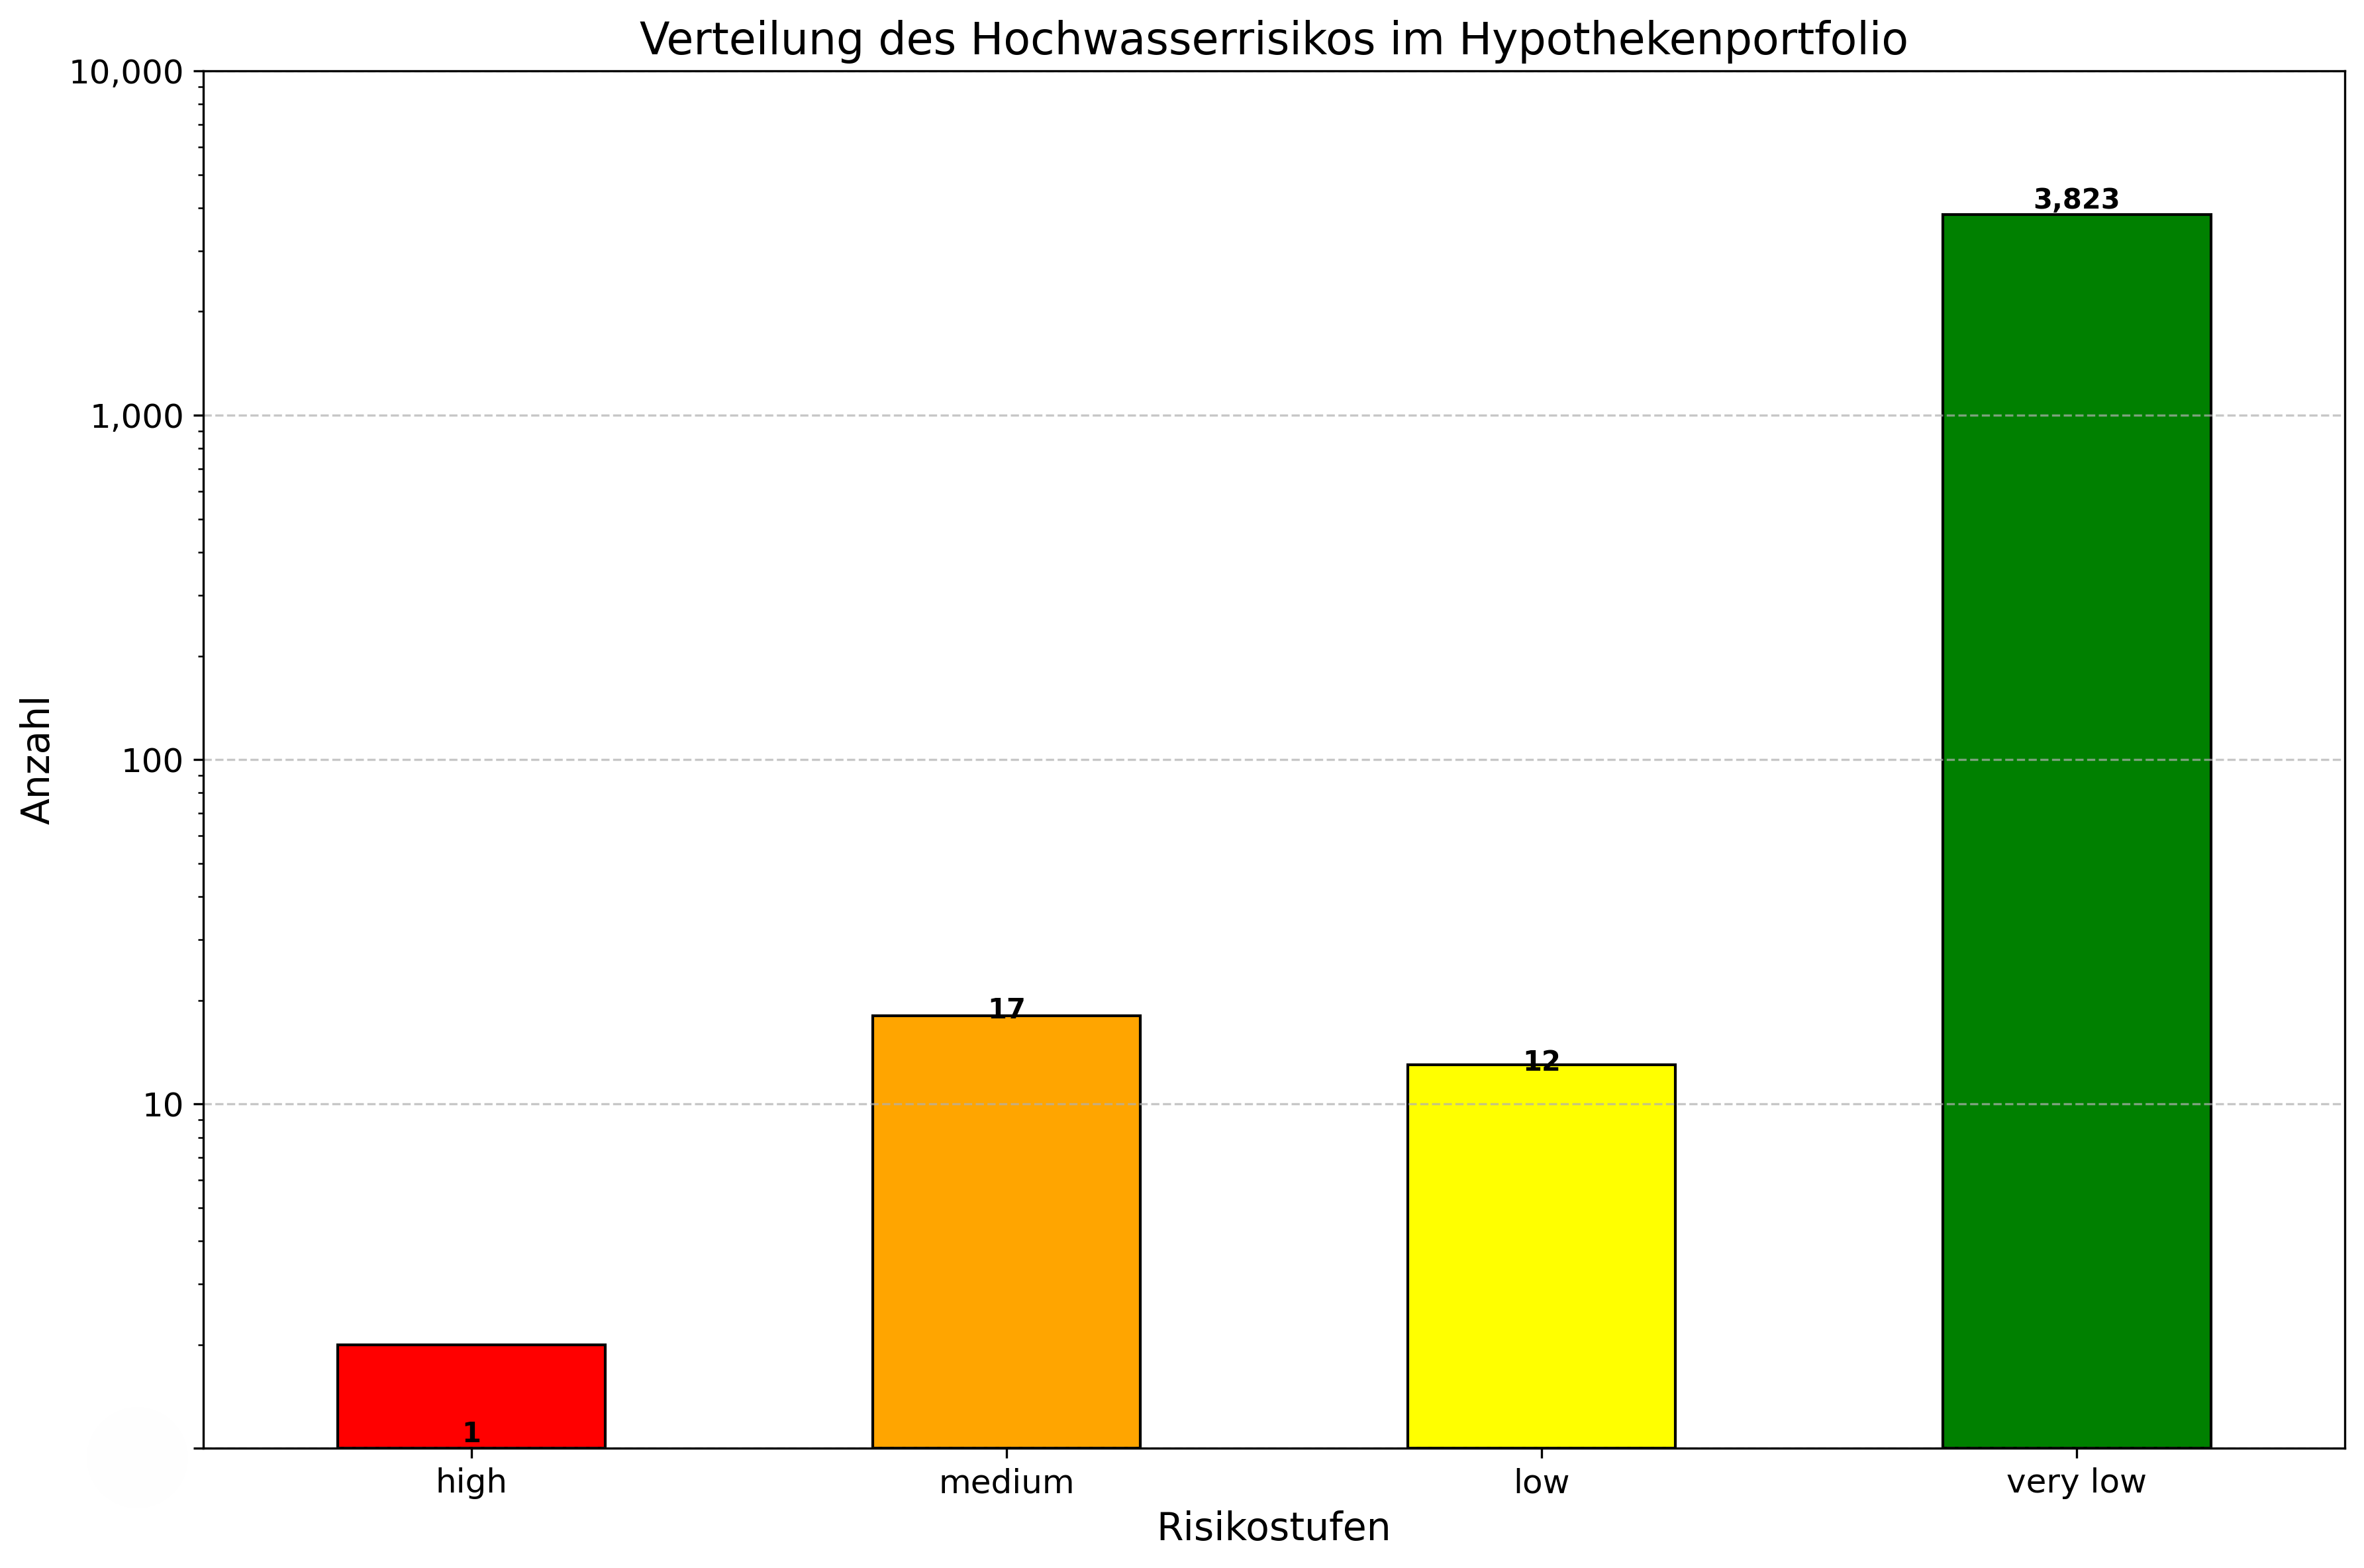
\includegraphics[width=0.8\textwidth]{figures/hochwasserrisiko_verteilung.png}
    \caption{Verteilung der Hochwasserrisikostufen im Hypothekenportfolio. Quelle: Eigene Darstellung}
    \label{fig:riskostufe}
\end{figure}
\FloatBarrier
Mittels des digitalen Geländemodells von Bayerns sowie Pegelnullpunkt und Hochwasserstand von \textcite{bayern2016hochwassernachrichtendienst} wurde die Überflutungstiefe bestimmt. Dies betrifft Datenpunkte in den Kategorien hoch, mittel und niedrig.
Aufgrund der Größe der \ac{DGM}-Daten (240 GB) erfolgte die Berechnung nur für 30 Punkte in Hochrisiko-, mittlerem und niedrigem Risikogebiet. Entsprechende Orts-, Gemeinde- und Landkreisdaten wurden geladen.
Im Hochrisikogebiet liegt ein einzelner Punkt in Haag an der Amper. Dort beträgt die maximale Überflutungstiefe 2,1 m, entsprechend einem Schadensfaktor von 0,16.
17 Datenpunkte befinden sich in Gebieten mittleren Risikos, verteilt auf verschiedene Orte.In der Kategorie mittleres Risiko gibt es Punkte mit einer Überschwemmungstiefe von 0. Dies ist durchaus plausibel. Innerhalb eines Gebiets mit mittlerem Risiko variiert die Topographie. Höher gelegene Standorte weisen eine geringere Überflutungstiefe auf. Ähnlich verhält es sich mit 12 Datenpunkten in Gebieten mit niedrigem Risiko. Auch dort können nicht-null Überschwemmungstiefen auftreten. Dies ist auf die niedrigere Geländehöhe zurückzuführen. 

Die Ermittlung der Tiefe für 3823 Datenpunkte in sehr niedrigen Risikogebieten wurde nicht durchgeführt. Diese Datenpunkte umfassen 1518 Orte, verteilt über 72 Landkreise. Eine individuelle Bewertung ist sehr aufwendig, da alle Kartendaten manuell geladen werden müssen und kein vollständiger Datensatz für Bayern mit Pegelnullpunkten und Hochwasserständen vorhanden ist. Diese Informationen müssen zudem auch manuell gesucht werden. Aufgrund dieser Einschränkungen wurden für alle Datenpunkte in sehr niedrigen Risikogebieten eine Überflutungstiefe und Schadensfaktor von 0 angenommen.

Nach der Berechnung der Überflutungstiefe kann durch den Vergleich mit der Schadenfunktion in Abbildung \ref{fig:damage_curve2} der entsprechende Schadensfaktor ermittelt werden. Basierend auf diesem Schadensfaktor lässt sich mithilfe der Gleichung \ref{eq:schaden} der Immobilienschaden quantifizieren. Die Resultate dieser Berechnungen für den Immobilienschaden werden anschließend in Abbildung \ref{fig:schadenwert} grafisch dargestellt.
\begin{figure}[htbp]
    \centering
    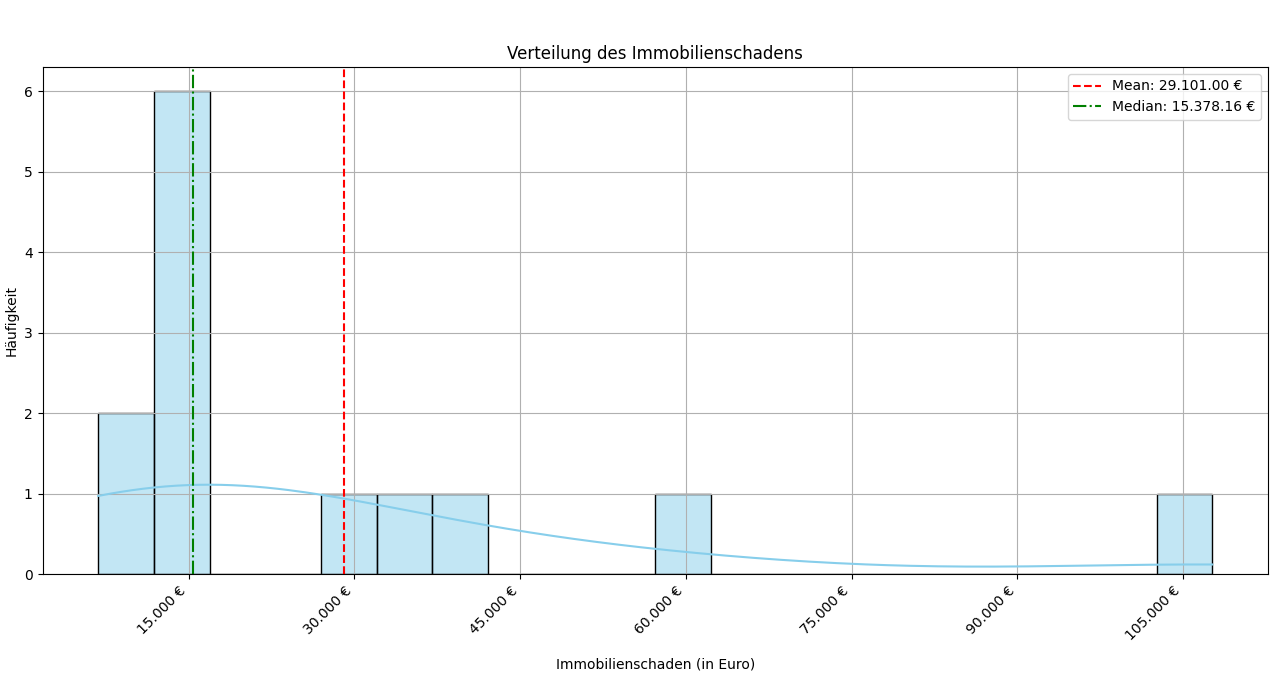
\includegraphics[width=\textwidth]{figures/flutschaden.png}
    \caption{Verteilung des Immobilienschaden im Hypothekenportfolio. Quelle: Eigene Darstellung}
    \label{fig:schadenwert}
\end{figure}
\FloatBarrier
Abbildung \ref{fig:schadenwert} zeigt eine rechtsschiefe Verteilung des Immobilienschadens, wobei die Mehrheit der Fälle im Bereich von etwa 8.000 bis 20.000 liegt. Der Median von 23.275,68 € liegt signifikant unter dem arithmetischen Durchschnitt von 35.558,03 €, was darauf hindeutet, dass es eine Ausreißer mit sehr hohen Schadensbeträgen gibt.


\begin{table}[htbp]
    \centering
    \caption{Hypothekenstatistik unter Berücksichtigung von Hochwasserschäden}
    \label{tab:hypothekenstatistiken}
    \small
    \begin{tabularx}{\textwidth}{>{\raggedright\arraybackslash}m{3.5cm}*{5}{>{\centering\arraybackslash}X}} 
    \toprule
    Metrik & Mean & Median & Min & Max & Std \\
    \midrule
    Akt. LtV & 0,4331 & 0,3400 & 0,1200 & 0,7100 & 0,1953 \\
    Neue LtV & 0,4785 & 0,5249 & 0,1220 & 0,7650 & 0,2092 \\
    Akt. ImmWert & 475.937,88 & 346.735,06 & 290.946,02 & 1.782.375,74 & 401.402,81 \\
    Neu. ImmWert & 440.379,85 & 308.751,00 & 267.372,00 & 1.728.904,47 & 396.910,80 \\
    Neue RWA & 43.140,48 & 42.174,46 & 15.015,81 & 72.381,12 & 20.672,58 \\
    Akt. RWA & 41.952,93 & 40.939,72 & 15.015,81 & 72.381,12 & 20.879,41 \\
    \bottomrule
    \end{tabularx}
\end{table}

Die Tabelle \ref{tab:hypothekenstatistiken} ist eine Zusammenfassung der Berechnungsergebnisse von Immobilienschäden, neuen LtV und RWA. Die Analyse zeigt signifikante Veränderungen in mehreren Finanzkennzahlen. Der durchschnittliche Loan-to-Value stieg von 43,31\% auf 47,85\%, was auf ein erhöhtes Kreditrisiko hindeutet. Dies resultiert aus der Wertminderung der Sicherheiten bei unverändertem Kreditbetrag. Der mittlere Immobilienwert sank von 475.937,88€ auf 440.379,85€, was die negativen Auswirkungen von Hochwasserrisiken auf den Vermögenswert verdeutlicht. Diese Entwicklung war in allen untersuchten Fällen zu beobachten. Die Risk-Weighted Assets zeigten einen leichten Anstieg im Durchschnitt von 41.952,93€ auf 43.140,48€. Obwohl dieser Anstieg nur in 15,38\% der Fälle auftrat, könnte er zu erhöhten Kapitalanforderungen für die Bank führen. Die durchschnittliche RWA-Änderung betrug 3,46\%. Diese Trends reflektieren sowohl Veränderungen im Immobilienmarkt als auch mögliche Anpassungen in der Risikobewertung und Kapitalpolitik der Finanzinstitute.

\subsection{Transitionsrisiko}